% Vorlesung vom 14.01.2016
\renewcommand{\ldate}{2016-01-14}
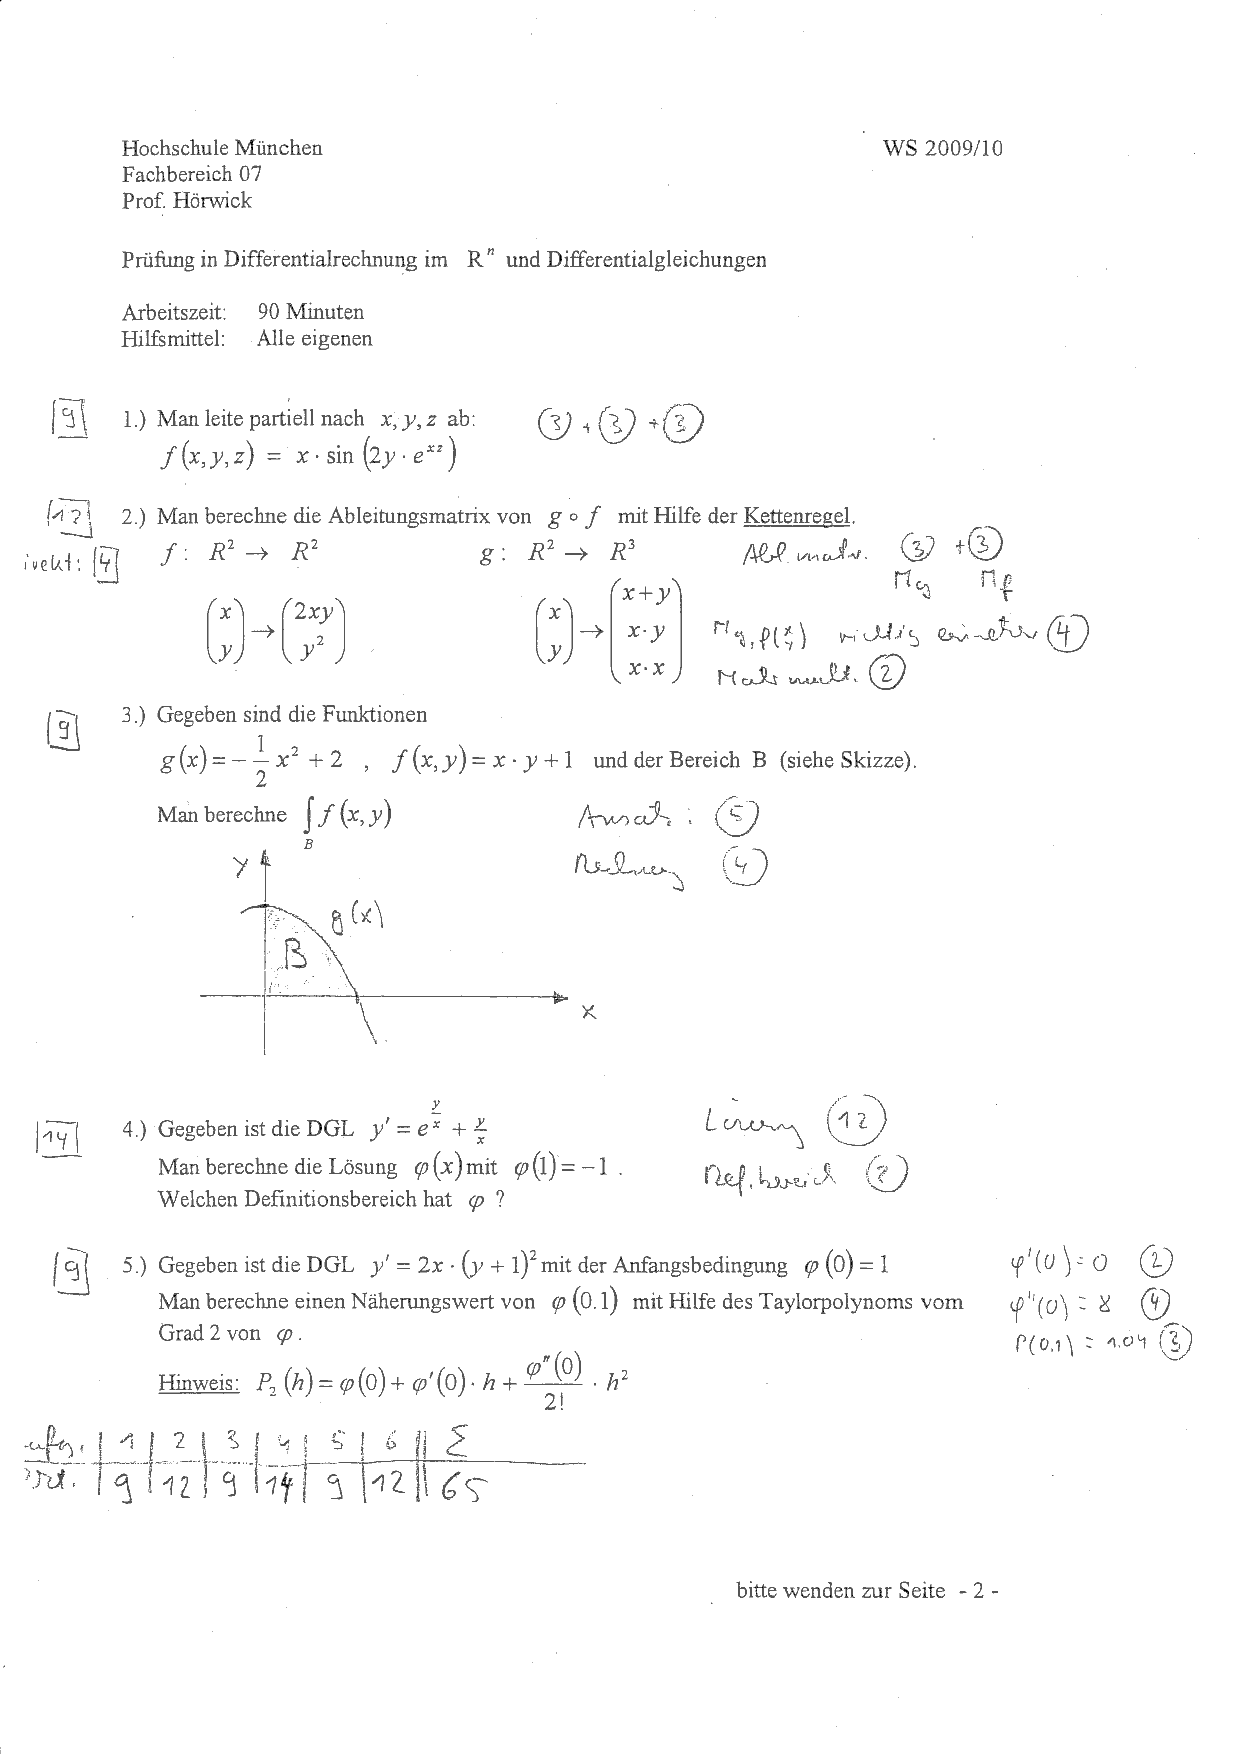
\includepdf[pages=-]{pruefungsangabe_diff_ws0910}

\section{Lösung für die Prüfung WS 2009/10}

\subsection{zu 1)}
$ f(x,y,z) = x \sin(2y e^{xz}) $ 

$ \frac{\df}{dx} = 1 \sin(2y\ e^{xz}) + x \cos(2y\ e^{xz}) 2y\ e^{xz} z $

$ \frac{\df}{dy} = x\cdot \cos(2y\ e^{xz}) \cdot 2e^{xz} $

$ \frac{\df}{dz} = x \cdot \cos(2y\ e^{xz}) \cdot 2y\ e^{xz} \cdot x $

\subsection{zu 2)}
$ f: \R^2 \rightarrow \R^2, \vektor{x\\y} \rightarrow \vektor{2xy\\y^2} $ und $ g: \R^2 \rightarrow \R^3, \vektor{x\\y} \rightarrow \vektor{x+y\\x\cdot y\\x\cdot x} $

$ (g\circ f)'(x) = g'(f(x)) \cdot f'(x) $

$ f'\vektor{x\\y} = \vektor{2y, 2x\\0, 2y} $

$ g'\vektor{x\\y} = \vektor{1, 1\\y, x\\2x, 0} $

$ (g\circ f)'\vektor{x\\y} = g' \rbr{f\vektor{x\\y}} \cdot f'\vektor{x\\y} 
= g'\vektor{2xy\\y^2} \cdot f'\vektor{x\\y}
= \vektor{1, 1\\y^2, 2xy\\4xy, 0} \cdot f'\vektor{2y, 2x\\0, 2y}
= \vektor{2y, 2x + 2y\\2y^3, 2xy^2 + 4xy^2\\8xy^2, 8x^2y, 0}
$

Kontrolle: Berechne $ g\circ f$, dann ableiten. 

\subsection{zu 3)}
\profnote{Doppelintegral. Grenze des ersten Integrals ist die Nullstelle, hier: 2.}
$
\int_{B} f
= \int_{0}^{2} \sbr{ \int_{0}^{g(x)} f(x,y) dy} dx 
= \int_{0}^{2} \sbr{ \int_{0}^{g(x)} x\cdot y + 1 dy} dx
$

$
= \int_{0}^{2} \sbr{ x\cdot \frac{1}{2} y^2 + y}_{y=0}^{g(x)=y=-\frac{1}{2} x^2 + 2} dx  
= \int_{0}^{2} \sbr{\frac{1}{2} x \cdot \rbr{-\frac{1}{2} x^2 + 2}^2 + \rbr{-\frac{1}{2} x^2 + 2} } dx
= ...
= 4
$

\subsection{zu 4)}
$ y' = \frac{y}{e^x} + \frac{y}{x} $ mit $\varphi(1) = -1$ und der Substitution 
$ z = \frac{y}{x},  y=z\cdot x, y' = z' \cdot x + z \cdot 1 \Rightarrow z' \cdot x + z = e^z + z \Leftrightarrow z' = \frac{1}{x} \cdot e^z$ (Typ: getrennte Variable)\\

Lösung $\psi, \psi(1) = \frac{-1}{1}=-1$:

$ \int_{z_0}^{\psi(x)} \frac{1}{e^t} dt = \int_{x_0}^{x} \frac{1}{t} dt$ \profnote{Jetzt brauchen wir eine Stammfunktion}

$ \sbr{- e^{-t}}_{\psi(1) = -1}^{\psi(x)} = \sbr{\ln \abs{t}}_1^x $ mit $x>0$

$ (-e^{-\psi(x)}) - (-e^1) = \ln x - \ln 1 $ \profnote{einsetzen}

$ -e^{-\psi(x)} = \ln x - e $ \profnote{Nach $\psi(x)$ auflösen}

$ e^{-\psi(x)} = e - \ln x $

$-\psi(x) = \ln (e- \ln x)$

$\psi(x) = - \ln (e- \ln x)$\\

Lösung $\varphi(x) = x\cdot \psi(x) $

$\varphi(x) = - x \ln(e - \ln x)$\\

Definition von $\varphi(x) : x > 0$

$e - \ln x > 0 $

$e > \ln x$

\underline{$ e^e > x > 0 $}

\subsection{zu 5)}
Eine ähnliche Aufgabe haben wir bereits gerechnet. 
